\chapter{CUDA shared memory避免bank conflict的swizzling机制解析}

\begin{center}\small 作者：frankshi（知乎 @frankshi-38）\quad 原文：\url{https://zhuanlan.zhihu.com/p/4746910252}\end{center}

\section{背景}

Cuda shared memory按照4字节一个bank，总共32个bank（128字节）来组织，其store和load操作在一定情况下存在bank conflict的情况：

\begin{itemize}
  \item 不同的线程访问同一bank的不同address时就会出现bank conflict。
  \item bank conflict只发生在同一个warp的不同线程间。
  \item 如果多个线程访问shared memory的相同bank的相同address，实际效果是broadcast，非bank conflict。
  \item bank conflict只发生在shared memory的读写操作上，global memory的读写操作不会有bank conflict产生。
\end{itemize}

\begin{quote}
在某些情况下，bank conflict的发生是在warp中处于同一个phase的不同threads之间，这里的phase是指warp的32个线程操作shared memory时，分多个phase，每个phase的参与线程不一样。比如ldmatrix指令\lstinline|ldmatrix.sync.aligned.x4.m8n8.shared.b16|，该指令从共享内存加载数据到线程寄存器，操作分4个phase，在phase0阶段，thread0~7操作共享内存，在phase1阶段，thread8~15操作共享内存，以此类推。
\end{quote}

bank conflict会导致warp被stall，冲突较多会对整个pipeline的耗时会有较大的影响。

\begin{quote}
当发生bank conflict时，warp需要额外的一个cycle来重新提交shared memory的访问指令到LSU单元，该指令需要在MIO中排队，这种排队会导致访问延迟增加，此时warp可能处于等待数据返回的状态，warp state标识为\textbf{Stall Short Scoreboard}。如果MIO队列满，此时warp先需要等待MIO队列处于非空的状态，此时warp state标识为\textbf{Stall MIO Throttle}。
\end{quote}

解决bank conflict的主要有下面几种：

\begin{itemize}
  \item padding。
  \item 转置存储（矩阵乘法的优化措施中，其中的一个典型操作是将从global memory读取的数据转置存储到shared memory中，本文中不做详细解释）。
  \item swizzling机制。
\end{itemize}

本文以矩阵转置这个kernel的实现为例，通过几种实现方法的对比，来解释swizzling机制是如何避免bank conflict。

\section{矩阵转置基于shared memory的naive实现}

下面是基于shared memory进行矩阵（矩阵大小：1028*2048）转置的一个naive实现：

\begin{lstlisting}
const int M = 1024; //矩阵行
const int N = 2048; //矩阵列
const dim3 block_size(32, 32);
const dim3 grid_size(N/32, M/32);
matrix_trans_shm<<<grid_size, block_size>>>(dev_A, M, N, dev_B);
\end{lstlisting}

kernel函数的实现如下：

\begin{lstlisting}
// 转置前的矩阵存储在dev_A中，矩阵大小为M*N，转置后的数据存储在dev_B中
__global__ void matrix_trans_shm(int* dev_A, int M, int N, int* dev_B) {
  int row = blockIdx.y * blockDim.y + threadIdx.y;
  int col = blockIdx.x * blockDim.x + threadIdx.x;

  // 每个block处理32*32的矩阵块
  __shared__ int s_data[32][32];

  if (row < M && col < N) {
    // 从全局内存中加载数据，转置后写到共享内存中
    s_data[threadIdx.x][threadIdx.y] = dev_A[row * N + col];
    __syncthreads();
    int n_col = blockIdx.y * blockDim.y + threadIdx.x;
    int n_row = blockIdx.x * blockDim.x + threadIdx.y;
    if (n_col < M && n_row < N) {
      // 从转置后的共享内存按行写到全局内存结果中
      dev_B[n_row * M + n_col] = s_data[threadIdx.y][threadIdx.x];
    }
  }
}
\end{lstlisting}

上述代码中声明的shared memory数组\lstinline|s_data[32][32]|，其中每个元素大小为4字节，刚好对应一个bank，而一行32个元素刚好对应完整的32个bank。数组中每个元素的对应的bank编号如下图所示：

\begin{figure}[htbp]\centering
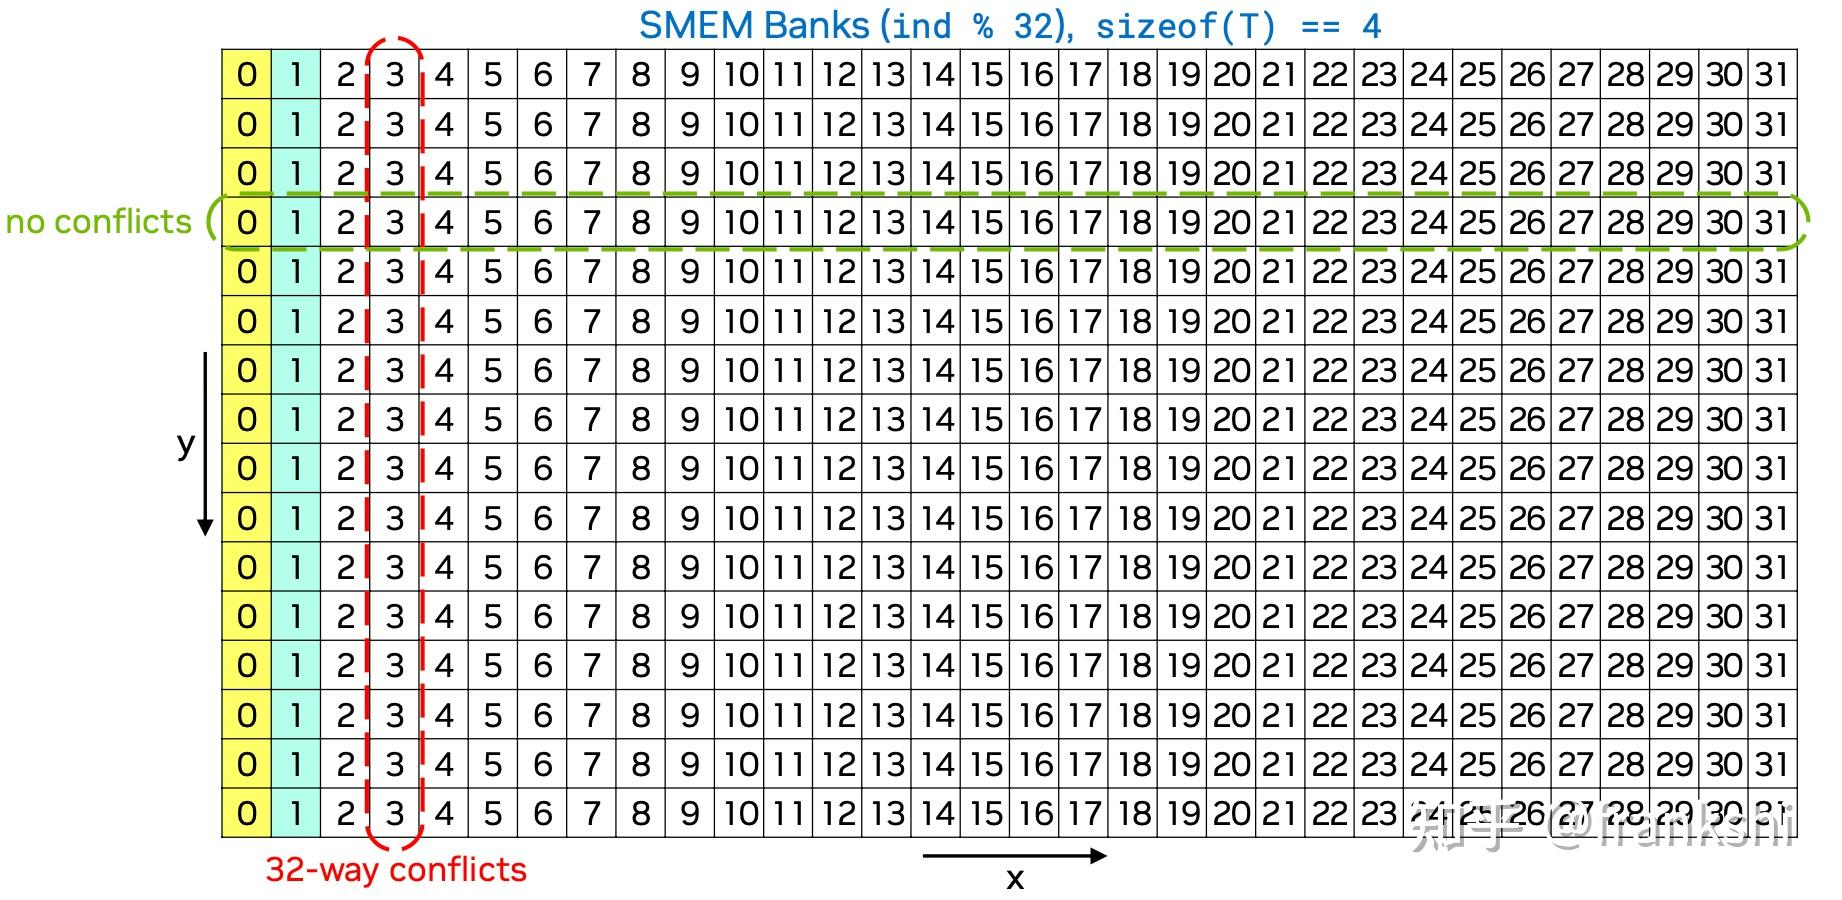
\includegraphics[width=0.9\textwidth]{figures/frankshi-01-swizzle/fig-01.jpg}
\end{figure}

\begin{quote}
上图中只显示了前16行信息，后续行省略。图片从这里截取：\href{https://www.nvidia.com/gtc/session-catalog/}{Advanced Performance Optimization in CUDA - NVIDIA GTC 2024}。
\end{quote}

warp是SM的基本执行单元，一个block内相邻的32个线程划分为一个warp，一个warp内的32个线程按照SIMT的模式来执行指令。在上述代码中，每个thread从global memory读取一个元素后，转置存储到shared memory中，对应到warp层面的实际的操作是：

\begin{itemize}
  \item warp先从global memory读取连续的32个元素（Colased access to global memory）。
  \item warp将读取的元素转置后写入到shared memory的同一列中。
\end{itemize}

可以看到，warp内的32个线程在写数据到shared memory数组中时，对应的同一列，这些地址全部落到相同的一个bank中，也就是32-way bank conflicts。通过profile的数据，可以看到 shared store的bank conflicts达到了2,032,616次。

\begin{figure}[htbp]\centering
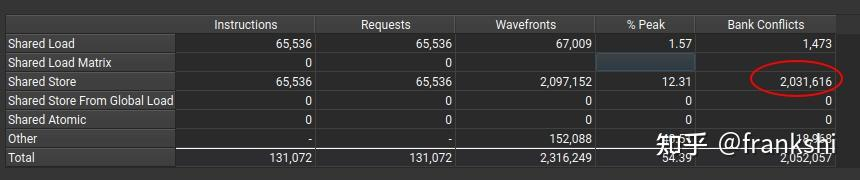
\includegraphics[width=0.9\textwidth]{figures/frankshi-01-swizzle/fig-02.jpg}
\end{figure}

\begin{quote}
说明：将转置后的数据从shared memory写入到输出内存时，是按\textbf{行}进行的load操作，理论上warp不应该存在bank conflicts，但上面的截图显示仍然有\textbf{1473}次冲突，推测这个load冲突跟我们的这里的读取逻辑无关。
\end{quote}

这个2,032,616次冲突的计算如下：

\begin{itemize}
  \item 每个warp的32个线程，第一个线程的写不会冲突，其他的31个线程的写都会冲突，因此每个warp的bank conflicts的次数为32-1=31。
  \item 每个block有32个warp，总的block数为(M*N)/(32*32)= (1024*2048)/(32*32) = 2048。
  \item 所有block累计的bank conflicts为2048(block)*32(warp)*31(conflicts) = 2031616。
\end{itemize}

类似的wavefronts的数值为2,097,152的计算如下：

\begin{itemize}
  \item 由于bank 冲突，32个线程的写都需要在MIO中排队，也就是需要分32次访问，每次访问对应一个wavefront(cycle)，如果没有冲突，32个线程只需要在MIO中排队一次，此时耗费的wavefronts数为1。
  \item 所有block累计的wavefronts = 2048(block)*32(warp)*32(wavefronts) = 2097152。
\end{itemize}

\begin{quote}
关于wavefront的概念：A \emph{wavefront} is the maximum unit that can pass through that pipeline stage per cycle. If not all cache lines or sectors can be accessed in a single wavefront, multiple wavefronts are created and sent for processing one by one, i.e. in a serialized manner.

A wavefront is described as a (work) package that can be processed at once, i.e. there is a notion of processing one wavefront per cycle in L1TEX. Wavefronts therefore represent the number of cycles required to process the requests, while the number of sectors per request is a property of the \emph{access pattern} of the memory instruction for all participating threads. For example, it is possible to have a memory instruction that requires 4 sectors per request in 1 wavefront. However, you can also have memory instruction having 4 sectors per request, but requiring 2 or more wavefronts.
\end{quote}

\section{使用Padding}

避免的bank conflict的一种方法是对shared memory使用padding，通过在尾部padding一个元素，数组变为\lstinline|s_data[32][33]|，这样相同列的不同行的元素的bank值不再一样，在转置时就避免了bank冲突。如下图所示：

\begin{figure}[htbp]\centering
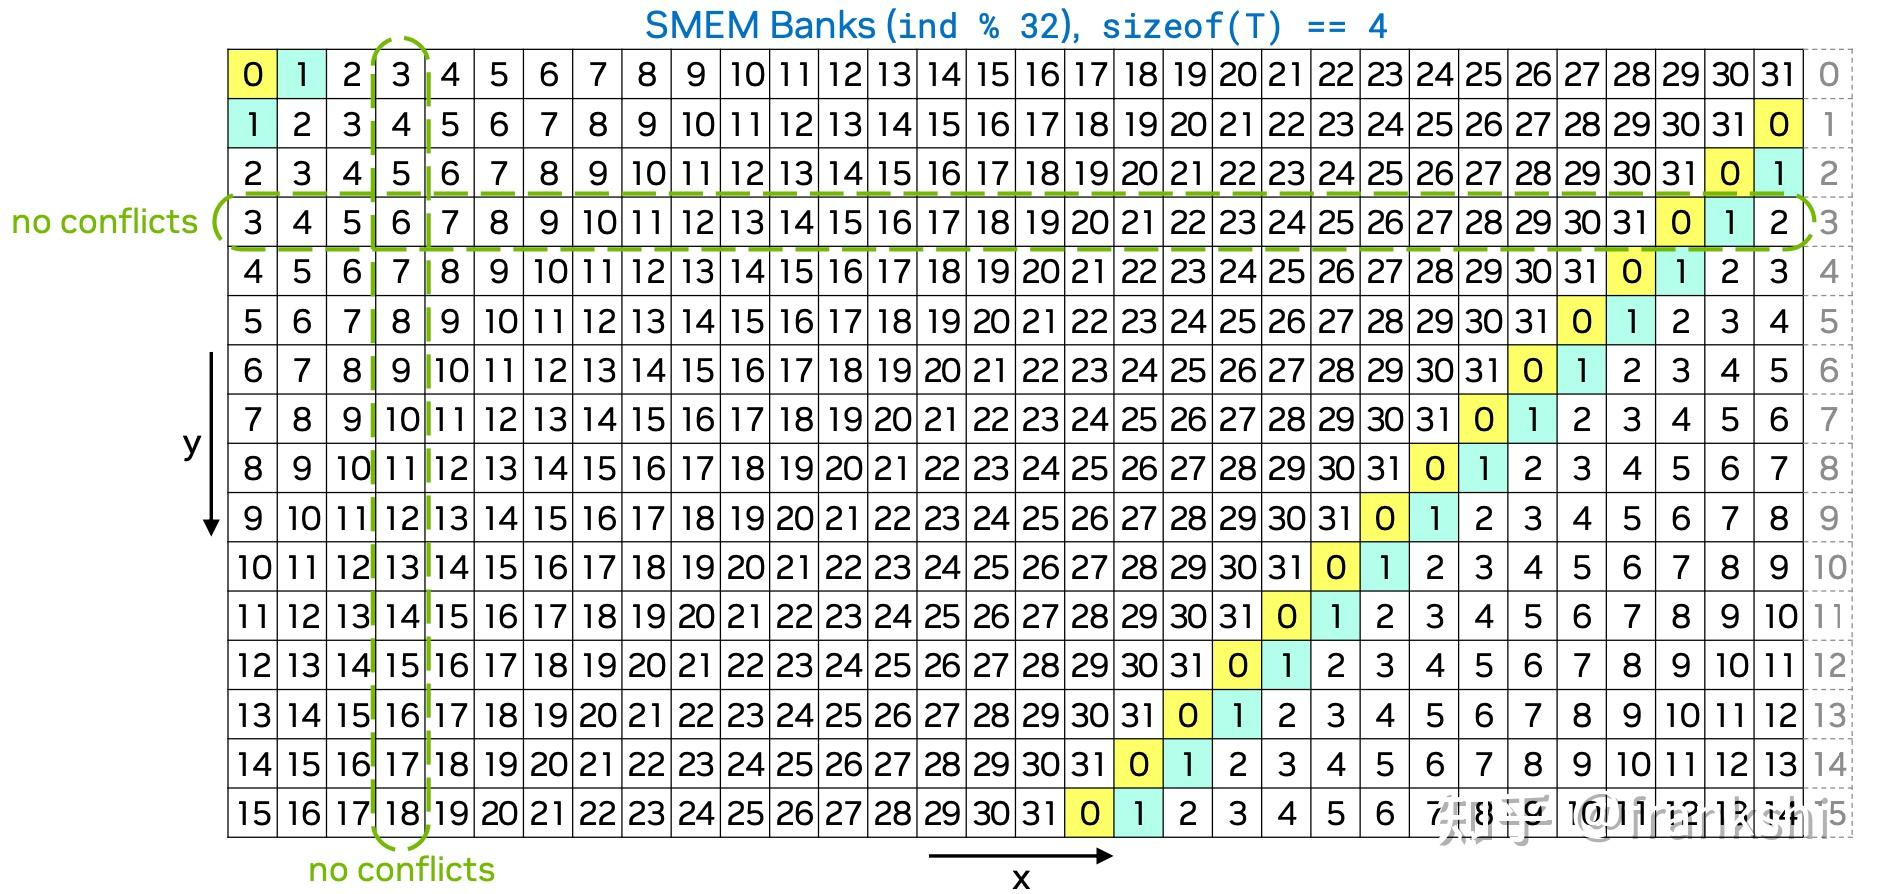
\includegraphics[width=0.9\textwidth]{figures/frankshi-01-swizzle/fig-03.jpg}
\end{figure}

新的代码如下：

\begin{lstlisting}
__global__ void matrix_trans_shm_padding(int* dev_A, int M, int N, int* dev_B) {
  int row = blockIdx.y * blockDim.y + threadIdx.y;
  int col = blockIdx.x * blockDim.x + threadIdx.x;

  // 每个block处理32*32的矩阵块，尾部padding来避免bank conflict
  __shared__ int s_data[32][33];

  if (row < M && col < N) {
    s_data[threadIdx.x][threadIdx.y] = dev_A[row * N + col];
    __syncthreads();
    int n_col = blockIdx.y * blockDim.y + threadIdx.x;
    int n_row = blockIdx.x * blockDim.x + threadIdx.y;
    if (n_col < M && n_row < N) {
      dev_B[n_row * M + n_col] = s_data[threadIdx.y][threadIdx.x];
    }
  }
}
\end{lstlisting}

profile的结果如下图所示，可以看出shared store的bank conflicts的数目变为0。

\begin{figure}[htbp]\centering
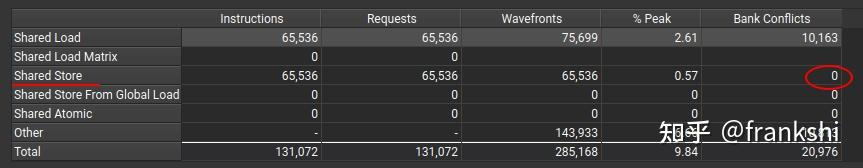
\includegraphics[width=0.9\textwidth]{figures/frankshi-01-swizzle/fig-04.jpg}
\end{figure}

padding的缺点有：

\begin{itemize}
  \item 可能降低SM的occupancy。由于每个SM的可使用的shared memory有限，如果每个block使用的共享内存增加，则SM内最大可并发的block数目减少，导致资源不能被充分利用，一些计算资源被闲置。
  \item 地址访问对齐问题。需要仔细考虑padding的大小来避免地址不对齐的问题，比如访问shared memory时可能是向量化的访问，比如\lstinline|int4|访问，也就是每次访问4个int，即16字节，那每次访问的地址必须是16字节对齐的，对于\lstinline|int s_data[32][33]|这种padding方式，第二行元素的起始地址就是非16字节对齐，会导致kernel执行出错。
\end{itemize}

\section{swizzling机制}

swizzling是在不额外分配内存的情况下，通过将shared memory的数据进行重排来避免bank conflict。下面是重排后的一个示例：

\begin{figure}[htbp]\centering
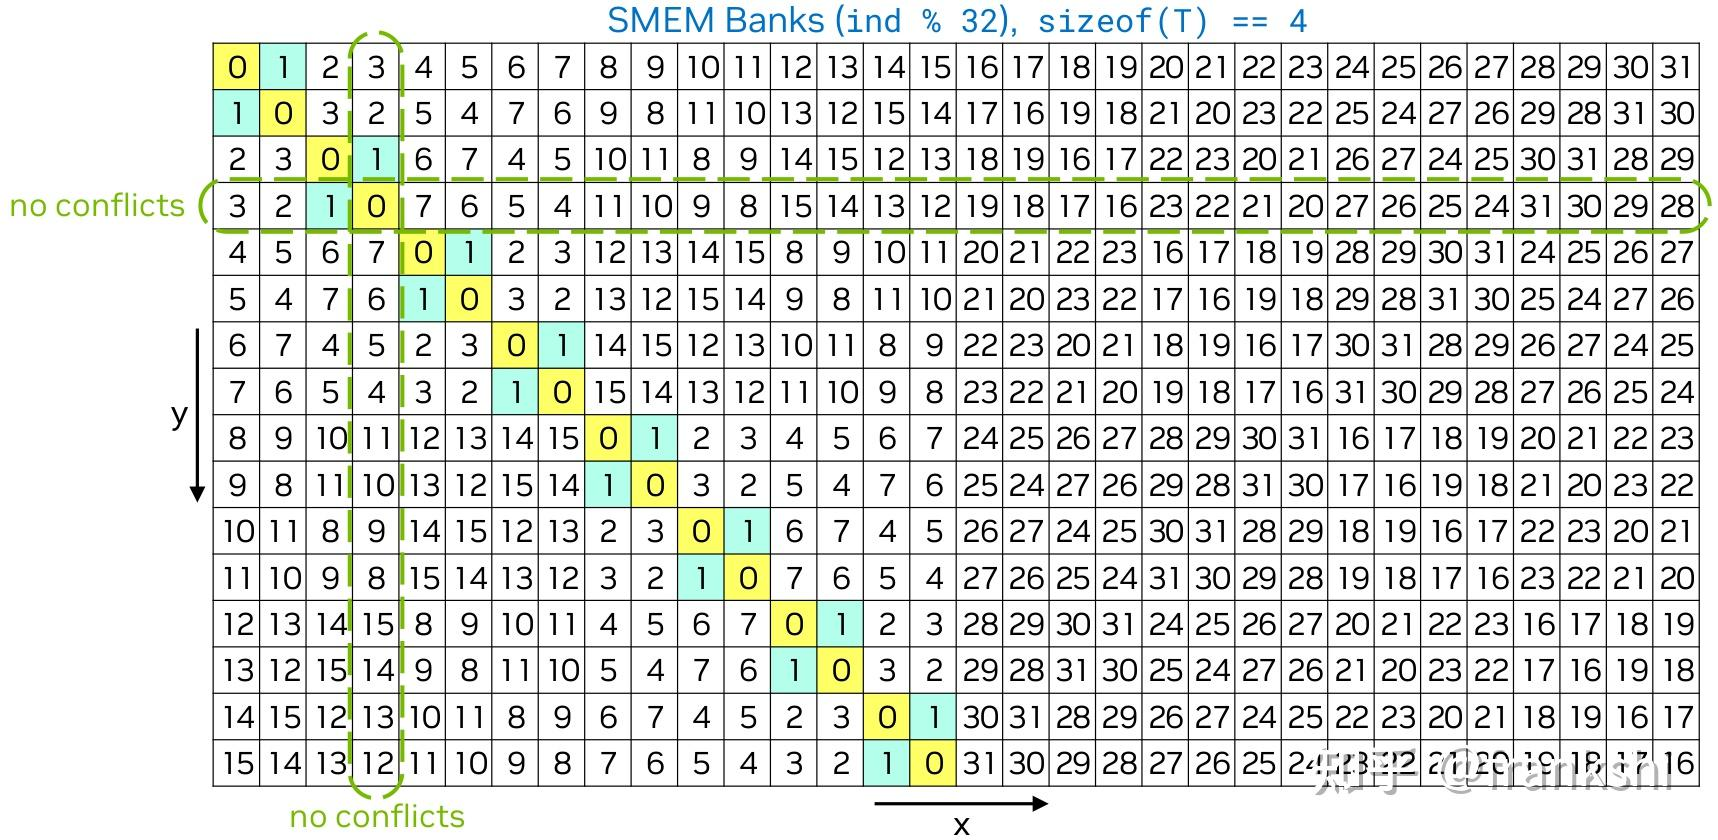
\includegraphics[width=0.9\textwidth]{figures/frankshi-01-swizzle/fig-05.jpg}
\end{figure}

在上面的图中，每个元素有唯一的位置信息 $(x, y)$ ， $x$ 和 $y$ 分别表示列和行，并且假设从0开始。
重排后，每一行内的数据集合保持不变，但行内元素的相对位置进行重排，比如对于 $y=1$ ，$x$原来的索引顺序是[0, 1, 2, 3, ......, 30, 31]，而新的索引顺序是[1, 0, 3, 2, 5, 4, ......, 31, 30]。
从上图可以看到，每一行/列的各个元素的bank值不再一样，这样就避免了shared memory在load/store操作时的bank冲突。

\subsection{4.1 逻辑位置和物理位置}

这里引入两个概念，逻辑位置和物理位置：

\begin{itemize}
  \item 逻辑位置表示元素在矩阵中的逻辑坐标。
  \item 物理位置表示其对应元素在实际存储数据的shared memory中的位置坐标。
\end{itemize}

当我们说读取矩阵的第2行第3列的元素，这里 $(x=3, y=2)$ 就表示逻辑位置，而真正读取数据的时候，我们需要从实际存储数据的shared memory中对应的位置 $(x=2, y=1)$ 去读取数据，这里逻辑坐标被映射到了shared memory中的物理坐标，如下图所示：

\begin{figure}[htbp]\centering
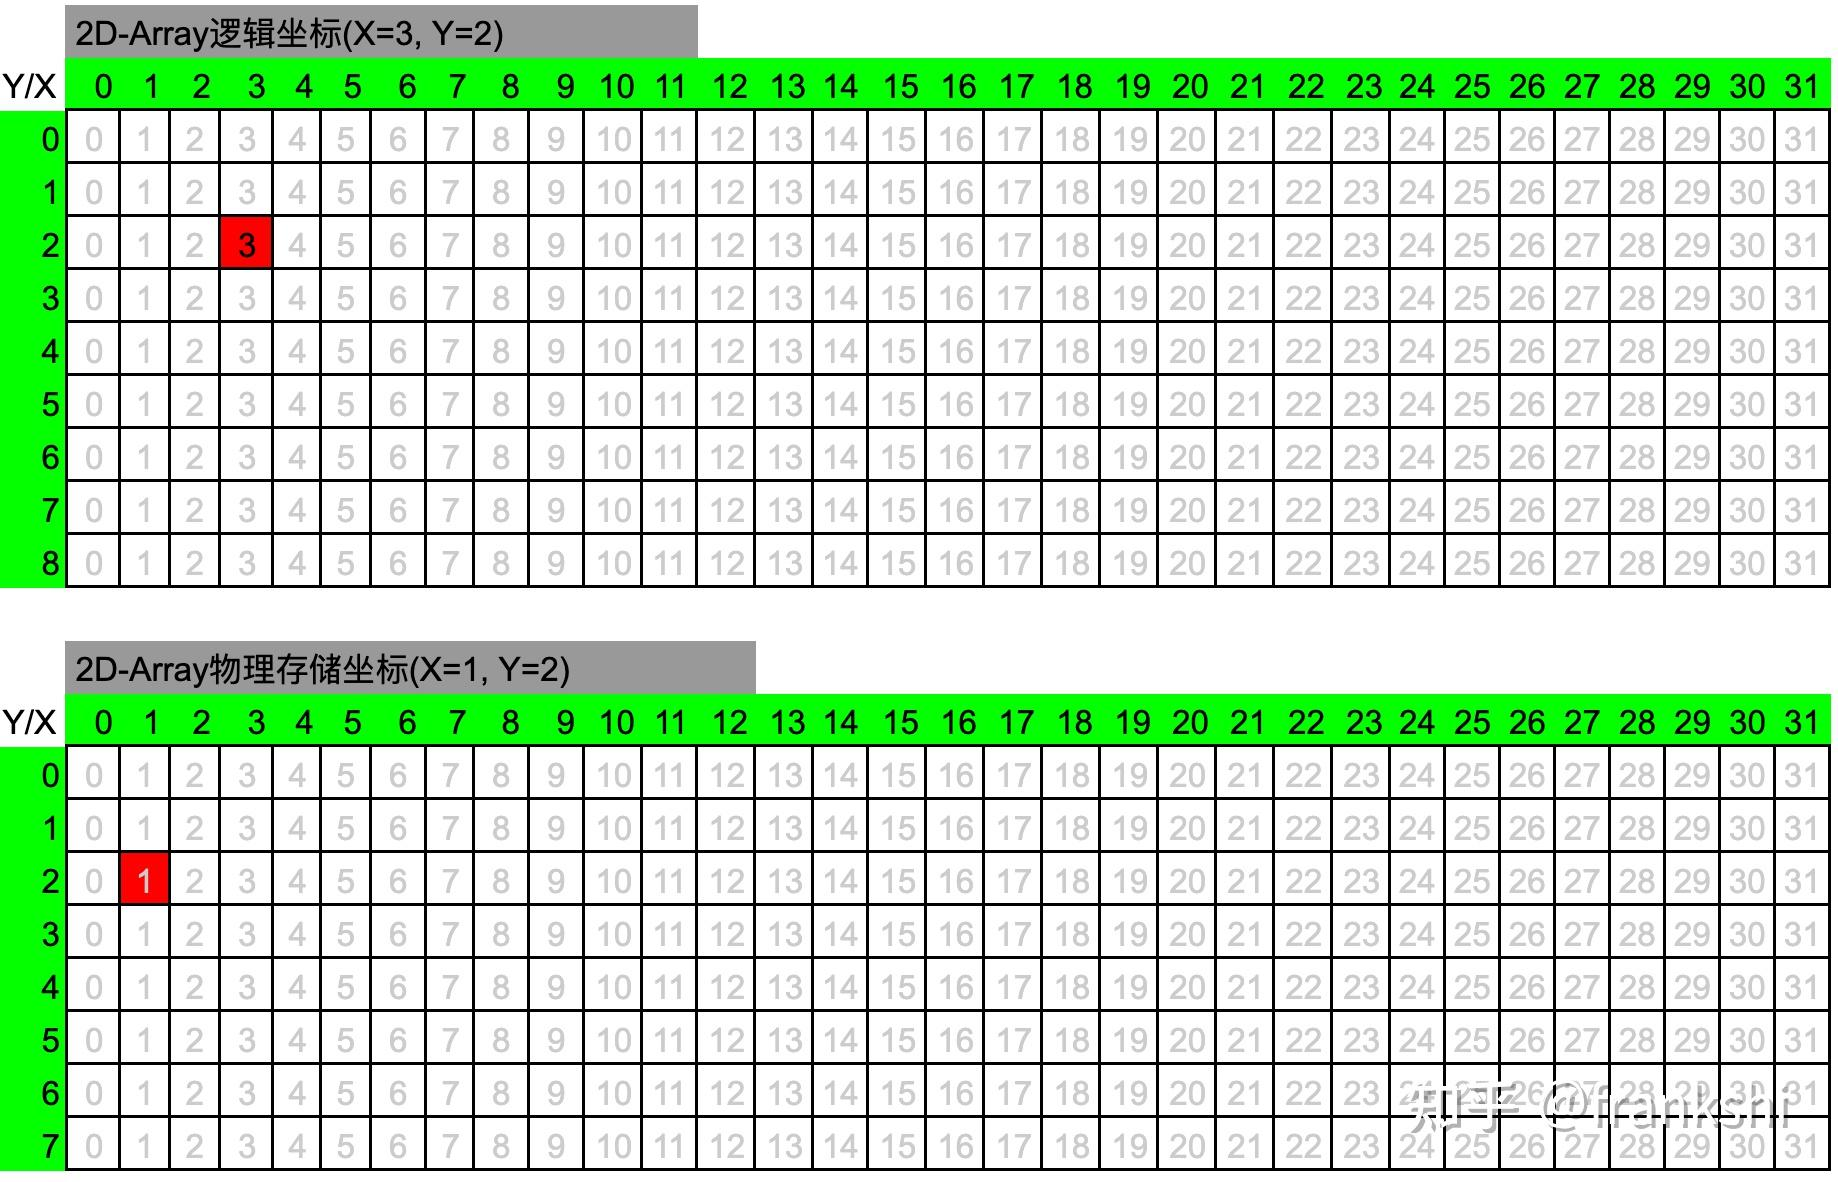
\includegraphics[width=0.9\textwidth]{figures/frankshi-01-swizzle/fig-06.jpg}
\end{figure}

在我们大部分的代码中，逻辑位置和物理位置是相同值，而在swizzling机制中，这两者不一样，存在一个映射关系：

\begin{equation*}
(x_p, y_p) = f(x_l, y_l)
\end{equation*}

上面的公式中 $(x_p, y_p)$ 表示物理存储坐标， $(x_l, y_l)$ 表示逻辑坐标， $x$ 和 $y$ 取值都是整数。这个映射必须满足：

\begin{itemize}
  \item 映射是一一对应的关系，即不能是多个逻辑坐标映射到同一个物理坐标或者一个逻辑坐标映射到多个物理坐标，否则就可能存在数据丢失或者重复的问题。
  \item 映射后的 $x$ 和 $y$ 的取值范围分别与映射前一致，否则可能会导致需要更多的shared memory容量，比如通过乘法映射也能满足一一映射关系，但映射后的值空间远大于映射前的范围。
\end{itemize}

\subsection{4.2 swizzling中的映射函数}

对于swizzling机制，逻辑坐标 $(x_l, y_l)$ 和物理坐标 $(x_p, y_p)$ 的映射关系如下：

\begin{itemize}
  \item $y_p = y_l$ ，物理行与逻辑行一致。
  \item $x_p = x_l \oplus y_l$ ，物理列等于逻辑行和逻辑列的异或值。
\end{itemize}

公式中的 $\oplus$ 表示异或操作，异或操作除了满足交换律和结合律之外，还有下面的一些性质：

\begin{itemize}
  \item 性质一： $x \oplus x = 0 $ 即两个相同的值进行异或，结果仍然为0。
  \item 性质二： $x \oplus 0 = x$ 即任何值与0进行异或，结果等于自身。
  \item 性质三：如果 $x_1 \neq x_2$ ，则 $x_1 \oplus x_2 \neq 0$ ，即两个不同的值异或，结果一定不为0。
  \item 性质四：如果 $x_1 \oplus x_2 \neq 0$ ，则 $x_1 \neq x_2$ ，即如果两个值异或的结果不为0，则两者的值一定不同。
\end{itemize}

下面将证明我们采用的这样映射满足4.1节中的条件。为了简化证明过程，我们在证明之前先附加下面的两个假设：

\begin{itemize}
  \item 条件一： $x$ 和 $y$ 取值范围一样。
  \item 条件二：$x$ 和 $y$ 的取值从0开始，最大取值为2的整数幂减去1，比如取值范围：[0, 31]。
\end{itemize}

实际的应用中，可能有些场景不满足上面的两个假设，但采用的映射函数核心思想与上面的映射类似，都是基于异或操作，但会针对不同的场景（向量化访问或者多phase访问）进行一些调整，在「TMA中的swizzling机制」一节中有相关的案例。

\subsection{4.3 一对一映射}

由于映射前后的坐标保持行不变，我们只需要证明，同行内两个不同列在映射后仍然保持列不同，即可证明坐标映射是一对一。
下面我们将证明同一行( $y$ 相同)的不同列( $x$ 不同)在映射后的 $x$ 值也不相等。
假设： $(x_{l1}, y),(x_{l2},y)$ 为同一行内的两个不同列的逻辑坐标，映射后的物理坐标为 $(x_{p1}, y),(x_{p2},y)$ 则有：

\begin{itemize}
  \item $x_{p1} = x_{l1} \oplus y$
  \item $x_{p2} = x_{l2} \oplus y$
  \item $x_{l1} \neq x_{l2} => x_{l1} \oplus x_{l2} \neq 0$
\end{itemize}

此时将 $x_{p1}$ 与 $x_{p2}$ 进行异或操作有：

\begin{equation*}
x_{p1} \oplus x_{p2} = (x_{l1} \oplus y) \oplus(x_{l2}\oplus y) = (x_{l1} \oplus x_{l2}) \oplus (y \oplus y) = (x_{l1} \oplus x_{l2}) \oplus 0 = (x_{l1} \oplus x_{l2}) \neq 0
\end{equation*}

根据异或的性质四得出： $x_{p1} \neq x_{p2}$ ，即同一行的两个不同逻辑坐标 $x$ 值在映射后的物理坐标 $x$ 值也不一样。
下面图显示 $y=3$ 的行内映射后的 $x$ 值各不一样：

\begin{figure}[htbp]\centering
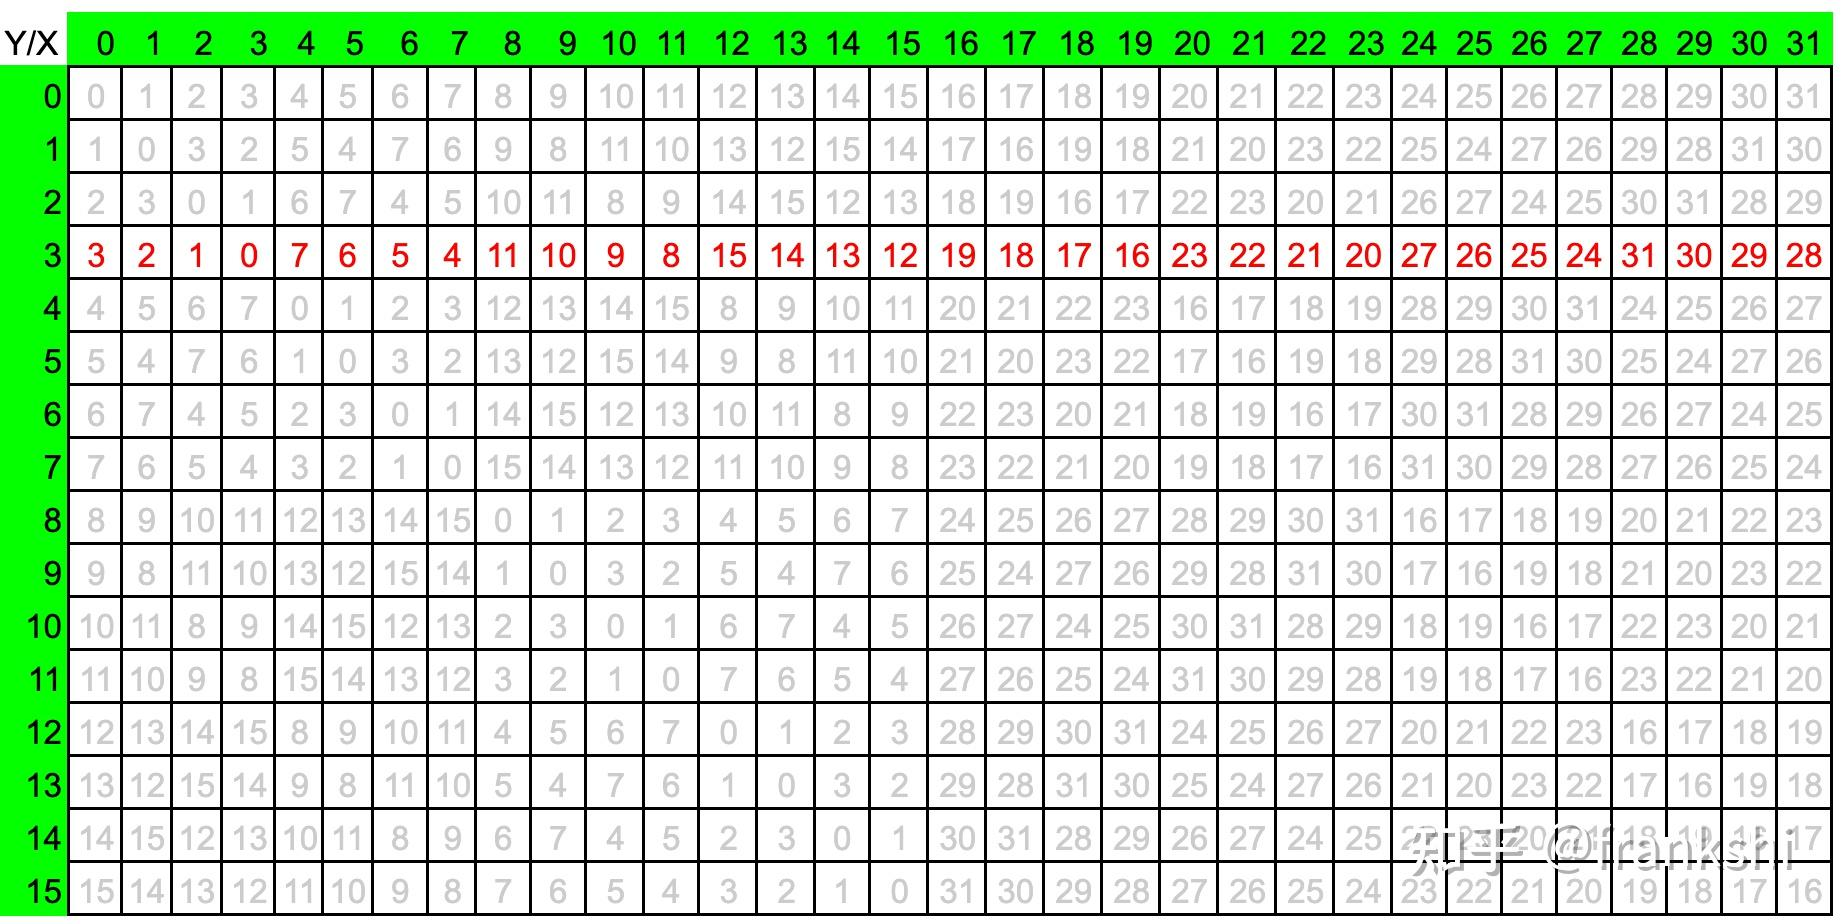
\includegraphics[width=0.9\textwidth]{figures/frankshi-01-swizzle/fig-07.jpg}
\end{figure}

反之，从映射后的物理坐标 $x_p$ 也能很容易的计算得到映射前的逻辑坐标 $x_l$ ，只需要将其与 $y$ 再进行异或：

\begin{itemize}
  \item $x_p \oplus y = (x_{l}\oplus y)\oplus y = x_{l} \oplus (y \oplus y) = x_{l} \oplus 0 = x_{l}$
\end{itemize}

\subsection{4.4 映射前后的取值范围保持不变}

还是以同一行( $y$ 相同)的不同列( $x$ 不同)在映射后的取值范围为例来说明。
由于映射前的 $x$ 的最大值为2的整数幂次方减1，对应的二进制表示的所有bit均为1，并且 $x$ 和 $y$ 的取值范围一致，故在该范围内，任意两个数异或后，最大可能值仍然为2的整数幂次方减1。
比如，对于 $(x,y)$ 取值范围均为[0, 31]来说，假设 $y$ 取值为3， $x$ 在0\textasciitilde{}31中，一定有：

\begin{itemize}
  \item 某个 $x = 3$ ，满足 $x \oplus y = 0$ 。
  \item 另外一个 $x =28$ ，满足 $x \oplus y = 31$ 。
\end{itemize}

另外，由于映射后的元素两两不一样，所以可以得出映射后的范围也是在0\textasciitilde{}31之间分布，即映射前后取值区间保持不变。

\subsection{4.5 列内任意两行在映射后的 $x$ 值不同}

现在我们将证明同一列( $x$ 相同)的不同行( $y$ 不同)在映射后的 $x$ 值也不相等。
假设： $(x, y_{l1}),(x,y_{l2})$ 为同一列内的两个不同行的逻辑坐标，映射后的物理坐标为 $(x_{p1}, y_{l1}),(x_{p2},y_{l2})$ ，则有：

\begin{itemize}
  \item $x_{p1} = x \oplus y_{l1}$
  \item $x_{p2} = x \oplus y_{l2}$
  \item $y_{l1} \neq y_{l2} => y_{l1} \oplus y_{l2} \neq 0$
\end{itemize}

$x_{p1}$ 和 $x_{p2}$ 的两者异或值为：

\begin{equation*}
x_{p1} \oplus x_{p2} = (x \oplus y_{l1}) \oplus(x \oplus y_{l2}) = (x \oplus x) \oplus (y_{l1} \oplus y_{l2}) = 0 \oplus (y_{l1} \oplus y_{l2}) = (y_{l1} \oplus y_{l2}) \neq 0
\end{equation*}

根据异或的性质四得出： $x_{p1} \neq x_{p2}$ ，即同一列的两个不同逻辑坐标 $y$ 值在映射后的物理坐标 $y$ 值也不一样。
另外，也很容易证明，映射后的某个行坐标值系列与对应的某个列值序列完全一致，比如：
 $y = 3$ 的行与 $x = 3$ 的列的值序列完全一致，如下图所示（下图只显示前16行）：

\begin{figure}[htbp]\centering
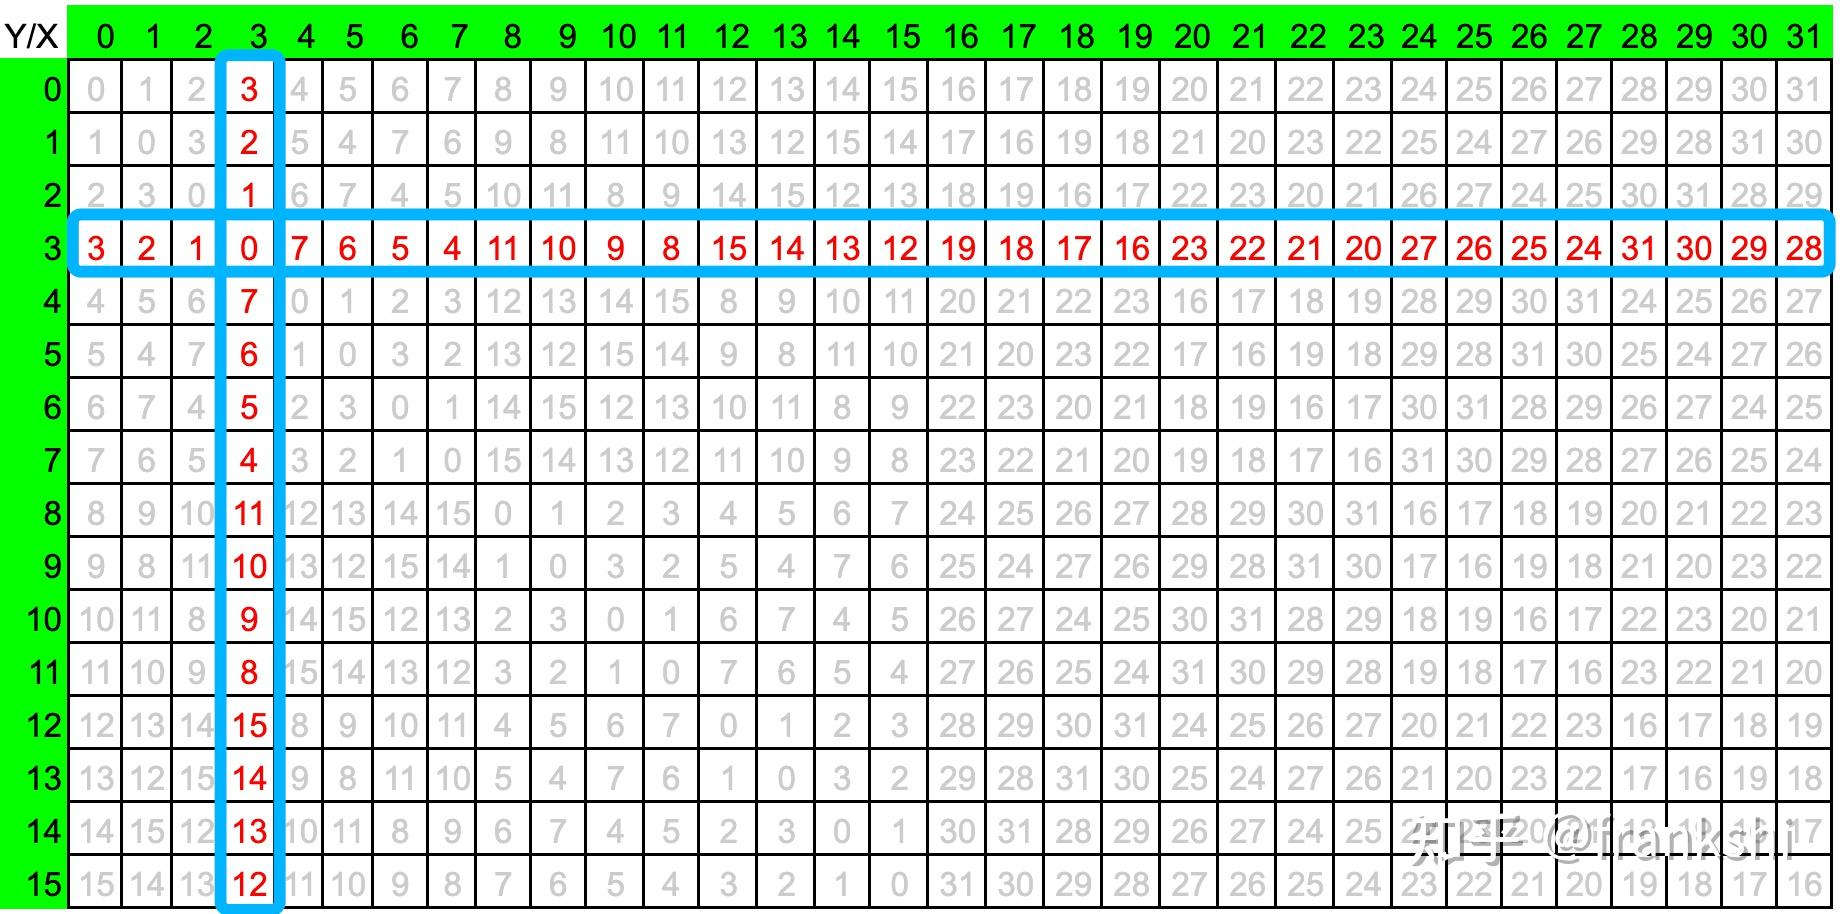
\includegraphics[width=0.9\textwidth]{figures/frankshi-01-swizzle/fig-08.jpg}
\end{figure}

从上面的证明过程看，在映射后，任意行和任意列内都不存在bank冲突了。

\subsection{4.6 swizzling机制的代码应用实践}

矩阵转置采用swizzling处理后的代码如下：

\begin{lstlisting}
__global__ void matrix_trans_swizzling(int* dev_A, int M, int N, int* dev_B) {
  int row = blockIdx.y * blockDim.y + threadIdx.y;
  int col = blockIdx.x * blockDim.x + threadIdx.x;

  __shared__ int s_data[32][32];

  if (row < M && col < N) {
    // 从全局内存读取数据写入共享内存的逻辑坐标(row=x,col=y)
    // 其映射的物理存储位置位置(row=x,col=x^y)
    s_data[threadIdx.x][threadIdx.x ^ threadIdx.y] = dev_A[row * N + col];
    __syncthreads();
    int n_col = blockIdx.y * blockDim.y + threadIdx.x;
    int n_row = blockIdx.x * blockDim.x + threadIdx.y;
    if (n_row < N && n_col < M) {
      // 从共享内存的逻辑坐标(row=y,col=x)读取数据
      // 其映射的物理存储位置(row=y,col=x^y)
      dev_B[n_row * M + n_col] = s_data[threadIdx.y][threadIdx.x ^ threadIdx.y];
    }
  }
}
\end{lstlisting}

代码中关于使用swizzling机制的代码逻辑如下：

\begin{itemize}
  \item 块中的每个线程从global memory读取一个元素后，在转置前，对应shared memory的逻辑为坐标\lstinline|(x = threadIdx.x, y = threadIdx.y)|，进行转置后存储的逻辑坐标为\lstinline|(x = threadIdx.y, y = threadIdx.x)|。
  \item 对于一个warp内的32个线程，\lstinline|threadIdx.y|值一样，\lstinline|threadIdx.x|不同，导致存储到shared memory中的位置是相同列不同行中，从而导致bank conflict。
  \item 此时，应用swizzling进行映射后的，转置存储时，行保持不变仍然为\lstinline|threadIdx.x|，新的列为 \lstinline|threadIdx.x ^ threadIdx.y|。
  \item 读取时采用类似的机制，将逻辑坐标转换为物理存储坐标，再从shared memory的对应物理位置去读。
\end{itemize}

Profile 结果如下：

\begin{figure}[htbp]\centering
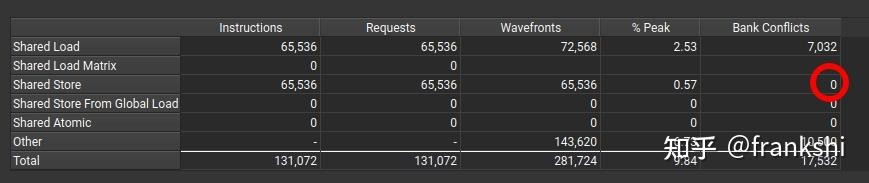
\includegraphics[width=0.9\textwidth]{figures/frankshi-01-swizzle/fig-09.jpg}
\end{figure}

图中显示shared memory store时bank conflicts=0，但load时还有bank conflict，推测跟swizzling无关。

\section{TMA中的swizzling机制}

\begin{quote}
TMA：Tensor Memory Accelerator，参考\href{https://docs.nvidia.com/cuda/hopper-tuning-guide/index.html#tensor-memory-accelerator}{这里}。
\end{quote}

矩阵乘法中，为了减少内存访问指令数目，通常通过向量化的访问指令来实现，比如\lstinline|int2/int4|，\lstinline|float2/float4|等，即一次访问8字节或16个字节。这种情况下，数据chunk的大小就不是4字节，跟单个bank的大小就不一样，此时仍然有bank冲突的现象存在，只是发生冲突的bank号不是连续分布，而是间隔分布，比如bank为0，4，8等等。为了避免冲突，可以按chunk为单位进行swizzling，其核心的处理思想仍然是使用异或操作，下图是一个示例：

\begin{figure}[htbp]\centering
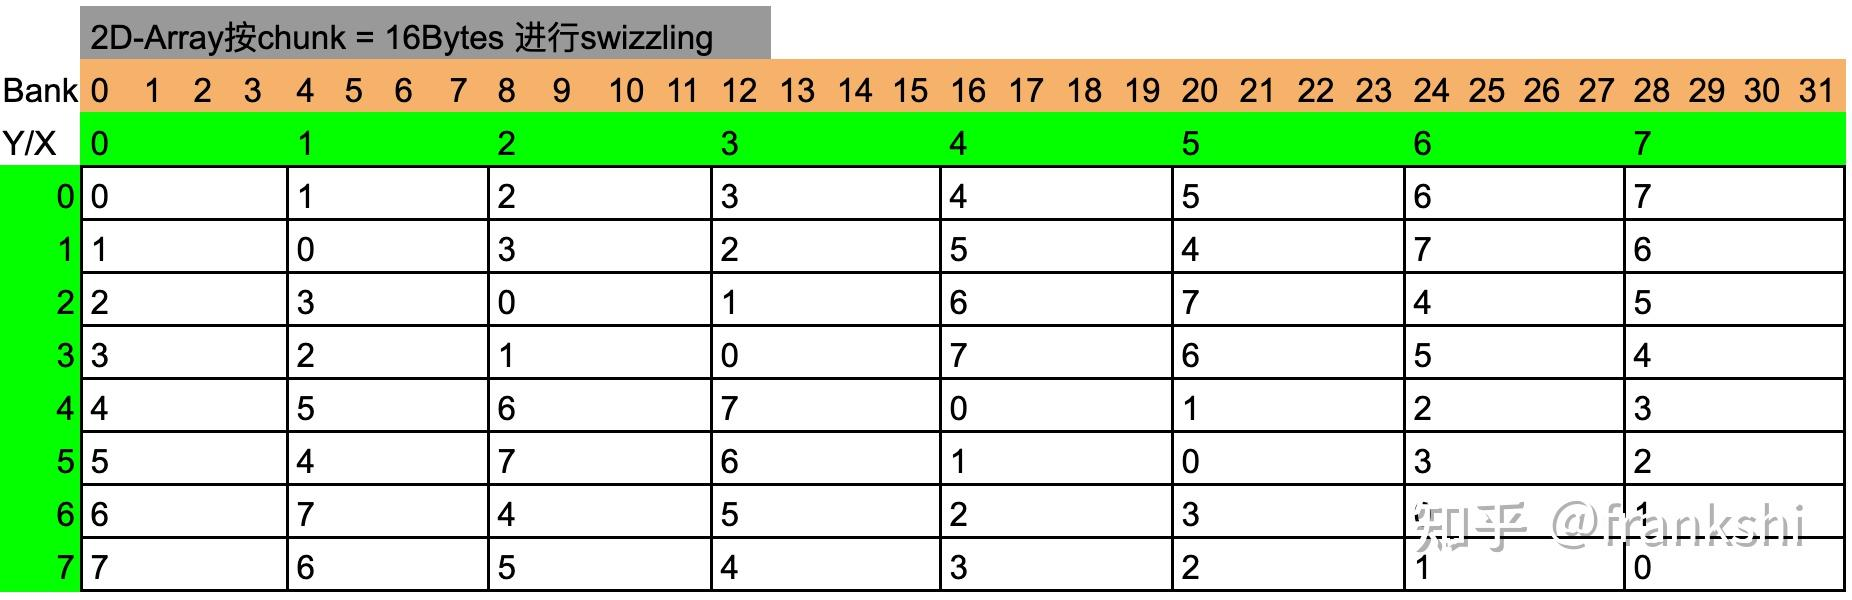
\includegraphics[width=0.9\textwidth]{figures/frankshi-01-swizzle/fig-10.jpg}
\end{figure}

下面说明TMA中进行swizzling的处理过程：

\begin{itemize}
  \item TMA以128字节单位为1个segment，以16字节为1个chunk。
  \item 通过对segment内的chunk进行swizzling，来实现不同segment间的bank conflict free。
\end{itemize}

TMA 假设使用的shared memory的数组的形式是\lstinline|T array[][NX]|（T可以是1/2/4Bytes的数据类型），并且满足：

\begin{itemize}
  \item \lstinline|NX * sizeof(T) == SWIZZLE_SIZE|。
  \item \lstinline|SWIZZLE_SIZE| 必须是32，64或者128三个值之一。
\end{itemize}

下面的计算过程假设\lstinline|SWIZZLE_SIZE=128|字节，对于数组中逻辑坐标是\lstinline|[y][x]|的元素，通过TMA映射后，在物理存储数组中的坐标为\lstinline|[y_swz][x_swz]|。跟之前的映射类似，物理坐标\lstinline|y_swz|与逻辑坐标y保持一致，\lstinline|x_swz|的计算过程如下：

\begin{itemize}
  \item 计算16字节的chunk块的索引
  \item \lstinline|i16 = (y * NX + x) * sizeof(T) / 16|。\lstinline|y16 = i16 / 8|。\lstinline|x16 = i16 % 8|。
  \item 计算这16字节的chunk块的swizzling的索引
  \item \lstinline|y16_swz = y16|，即chunk块的行保持不变。\lstinline|x16_swz = y16^x16|，即chunk块的列为逻辑行和逻辑列的异或值。
  \item 计算chunk块的某个x元素的映射后的索引
  \item 先计算chunk块在行内的偏移，然后计算chunk块中的元素在chunk块中的偏移，两者之和即为偏移。\lstinline|x_swz = x16_swz * 16 / sizeof(T) % NX + x % (16 / sizeof(T))|。
\end{itemize}

对于不同的\lstinline|SWIZZLE_SIZE|进行坐标重排后的其效果如下：

\begin{figure}[htbp]\centering
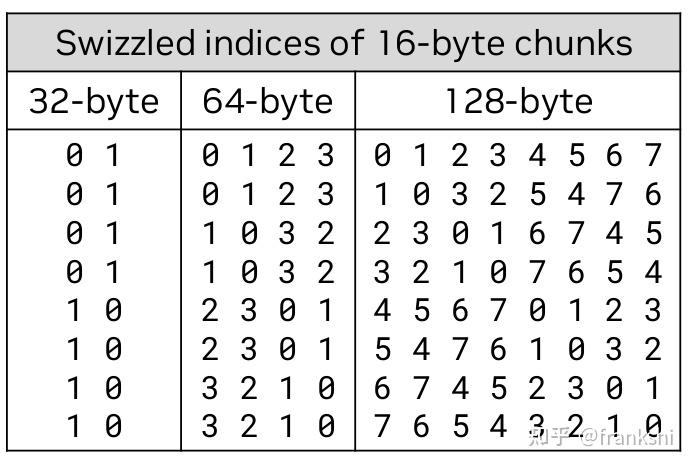
\includegraphics[width=0.9\textwidth]{figures/frankshi-01-swizzle/fig-11.jpg}
\end{figure}

由于\lstinline|SWIZZLE_SIZE|为128字节时，刚好对应了32个bank的大小，此时在chunk层面的进行的swizzling映射不会改变chunk所在的行，只会改变列。如果\lstinline|SWIZZLE_SIZE|不为128字节时，映射后有可能改变行，比如对于\lstinline|float4 array[15][4]|这样的数组，\lstinline|SWIZZLING_SIZE = 64|字节，对于数组中超过第8行的那些数据，第8行后的chunk块的前4个和后4个的相对位置已经发生变化，如下图所示：

\begin{figure}[htbp]\centering
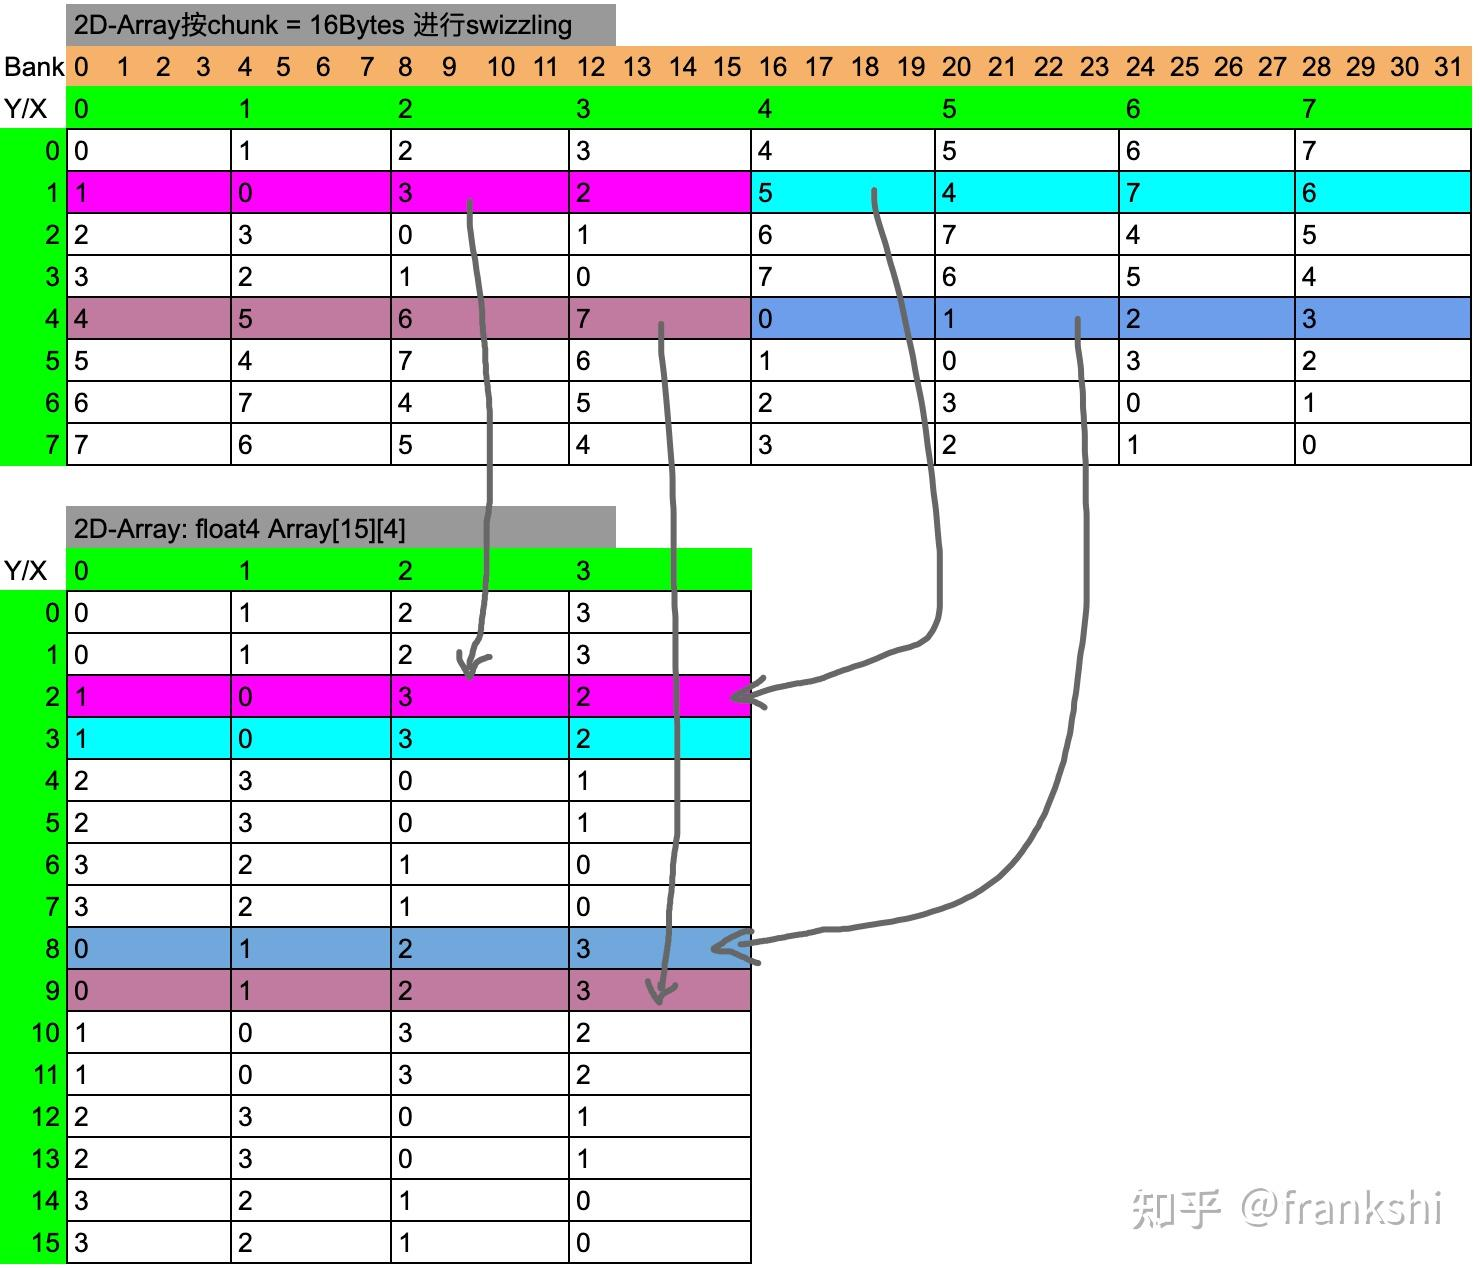
\includegraphics[width=0.9\textwidth]{figures/frankshi-01-swizzle/fig-12.jpg}
\end{figure}

对\lstinline|SWIZZLING_SIZE|不为128字节的情况，chunk的处理逻辑与上面的处理过程类似，但从chunk到单个元素的转换时，需要做些调整。

\section{Cutlass中的swizzling使用}

Cutlass 使用tensor core的进行矩阵乘法时，比如对于\lstinline|m16n8k16|的fp16的矩阵乘法，需要分4个phase从shared memory分别加载4个8x8的fp16的矩阵数据到线程寄存器中，此时的bank conflict只局限同phase的8个线程内，可以只考虑针对这8个线程需要访问的shared memory来进行swizzling，从而避免bank conflict，感兴趣的读者可以去找资料学习。

\begin{figure}[htbp]\centering
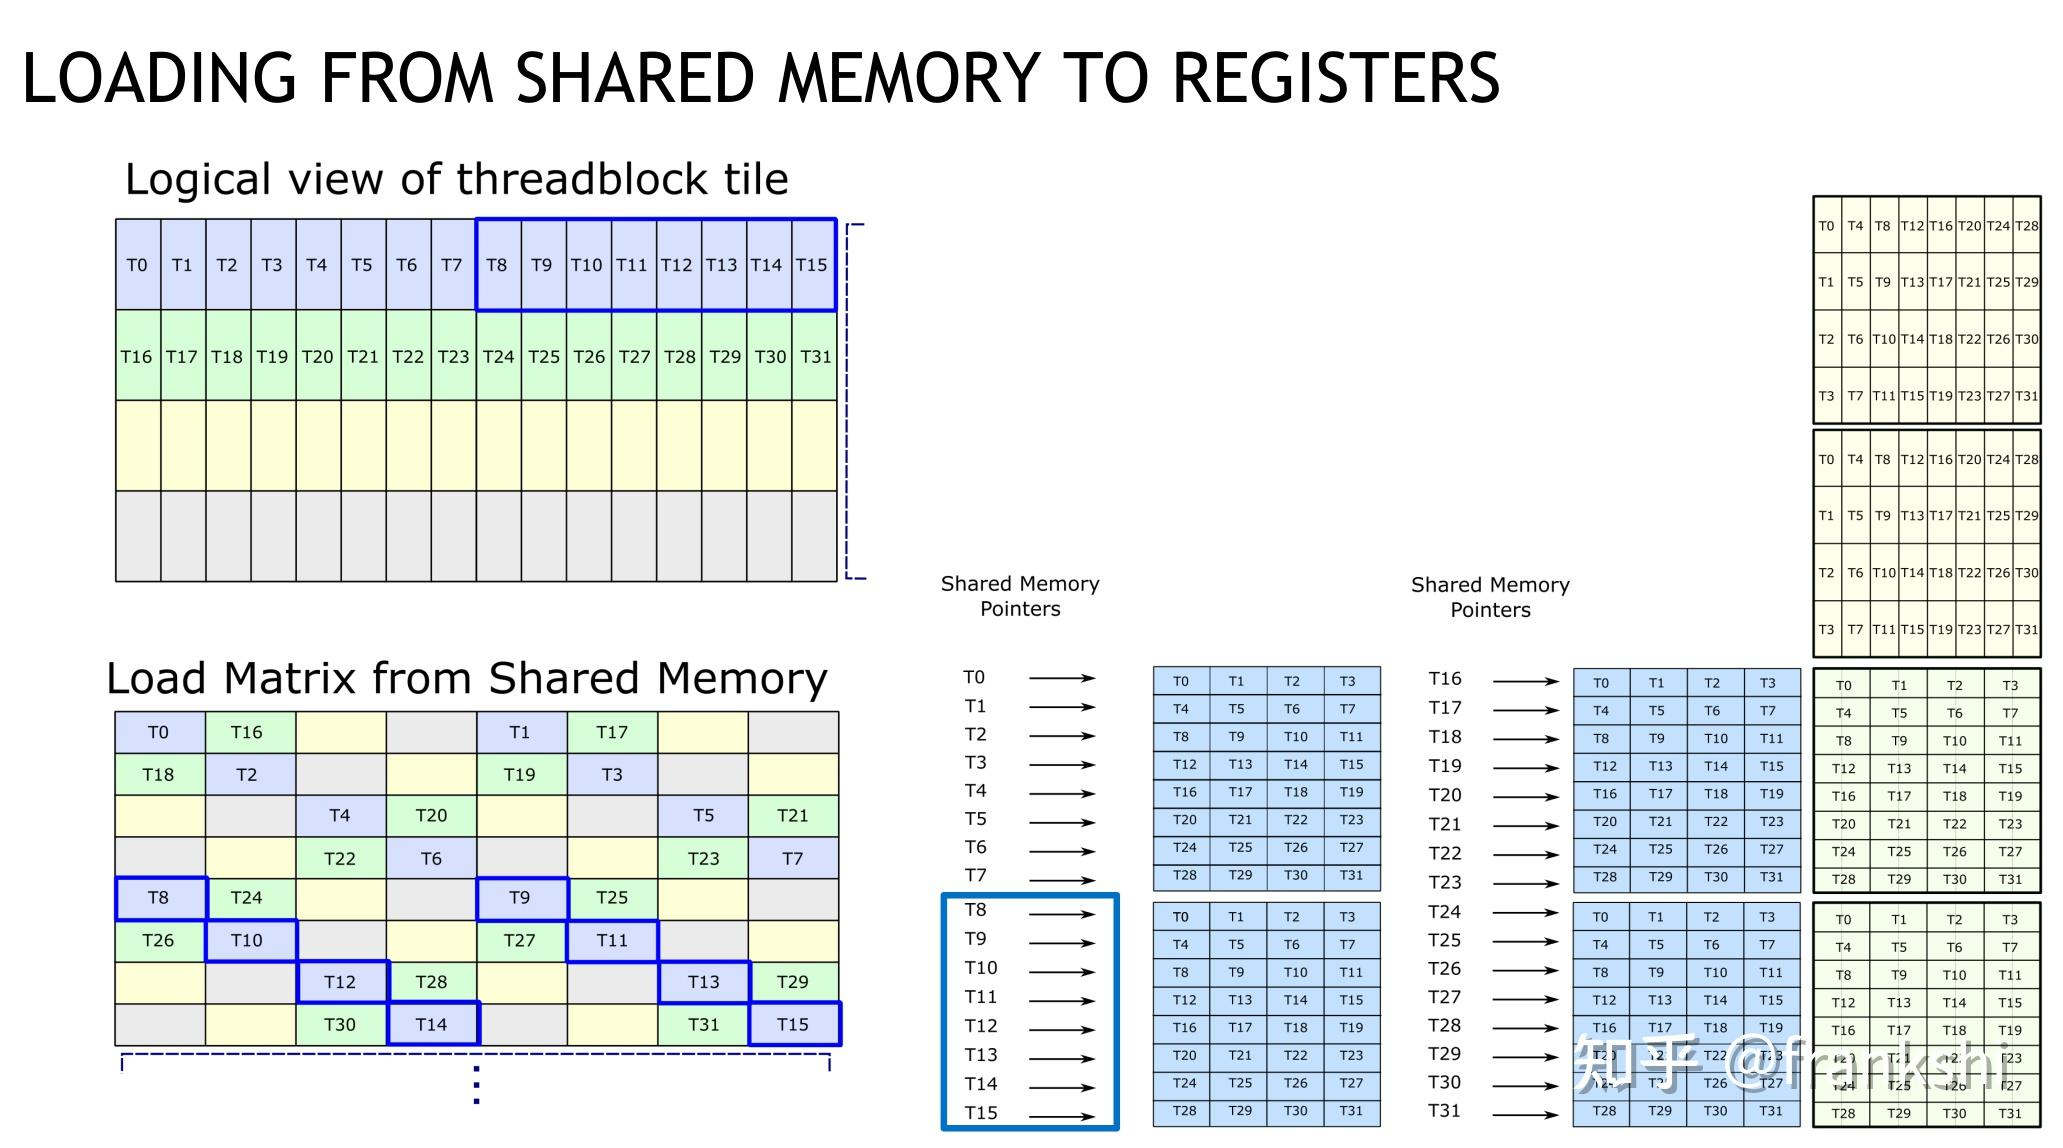
\includegraphics[width=0.9\textwidth]{figures/frankshi-01-swizzle/fig-13.jpg}
\end{figure}

\section{参考资料}

\begin{itemize}
  \item Advanced Performance Optimization in CUDA - NVIDIA GTC 2024 \url{https://www.nvidia.com/gtc/session-catalog/?search.h1topich1pppacceleratedcomputingtoolstechniquesp=1699467437927003C0hc#/session/1695395019805001m1oR}
  \item \url{https://www.nvidia.com/en-us/on-demand/session/gtcsj20-s21745/}
  \item \url{https://leimao.github.io/blog/CUDA-Shared-Memory-Swizzling/}
  \item \url{https://zhuanlan.zhihu.com/p/710337546}
\end{itemize}
